\documentclass[aps,reprint,superscriptaddress,10pt]{revtex4-2}
\usepackage{kotex}
\usepackage[HWP]{dhucs-interword}
\usepackage[dvips]{color}
\usepackage{graphicx}
\usepackage{bm}
\usepackage{amsmath}
\usepackage{tikz}
\usepackage{mhchem}
\usepackage{booktabs}
\usepackage{multirow}
\usepackage{array}
\usepackage{tikz}

\begin{document}
\title{응집물질물리실험 예비보고서 \\
\small 실험주제 : Photo lithography}

\author{HuiJae-Lee}\email{hjlee6674@inha.edu}
\affiliation{Physics Department, Inha University}

\date{\today}


\begin{abstract}
Photo lithography 공정을 직접 진행해보고 공정의 과정과
photo mask, photoresist, etching, depostion 등 공정에 필요한 요소들을 알아본다.
 \end{abstract}
 
 \maketitle
 
\section[Introduction]{Introduction}
Photo lithography는 반도체의 실제 회로를 만드는 과정이다.
반도체의 표면에 감광액을 바르고 자외선을 조사하여 감광액에 화학적 변화를 일으킨다.
이 때 조사하는 자외선은 포토마스크로 걸러지는데 이 포토마스크는 회로 패턴에 맞게
자외선을 걸러낸다. 포토마스크의 패턴에 맞게 자외선에 조사되어 감광액에 변화가 일어나면
더이상 필요하지 않은 감광액을 제거하여 반도체의 표면에 회로 패턴을 새기는 과정으로
진행한다(FIG.~\ref{fig:1}).
\begin{figure}[htbp]
  \centering
  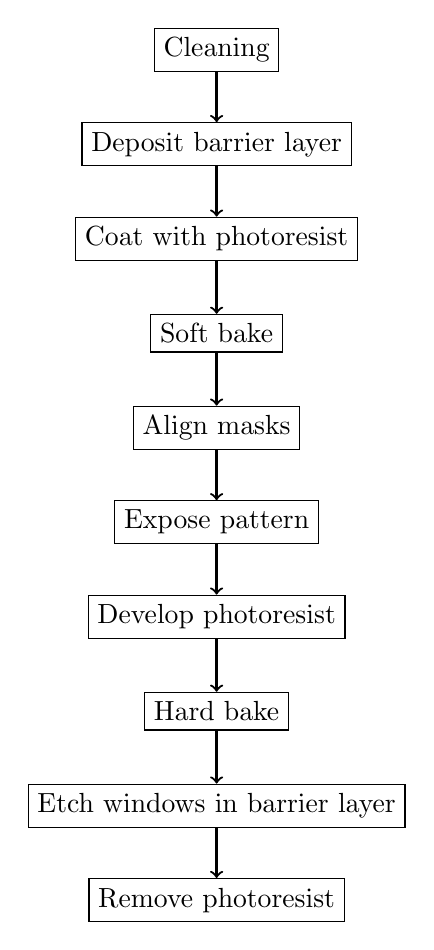
\begin{tikzpicture}
    \def \d {1.2};
  \node[draw, shape=rectangle](A) at (0,0)     {Cleaning};
  \node[draw, shape=rectangle](B) at (0,-\d)   {Deposit barrier layer};
  \node[draw, shape=rectangle](C) at (0,-2*\d) {Coat with photoresist};
  \node[draw, shape=rectangle](D) at (0,-3*\d) {Soft bake};
  \node[draw, shape=rectangle](E) at (0,-4*\d) {Align masks};
  \node[draw, shape=rectangle](F) at (0,-5*\d) {Expose pattern};
  \node[draw, shape=rectangle](G) at (0,-6*\d) {Develop photoresist};
  \node[draw, shape=rectangle](H) at (0,-7*\d) {Hard bake};
  \node[draw, shape=rectangle](I) at (0,-8*\d) {Etch windows in barrier layer};
  \node[draw, shape=rectangle](J) at (0,-9*\d) {Remove photoresist};

  \draw[->, thick] (A) -- (B);
  \draw[->, thick] (B) -- (C);
  \draw[->, thick] (C) -- (D);
  \draw[->, thick] (D) -- (E);
  \draw[->, thick] (E) -- (F);
  \draw[->, thick] (F) -- (G);
  \draw[->, thick] (G) -- (H);
  \draw[->, thick] (H) -- (I);
  \draw[->, thick] (I) -- (J);
  \end{tikzpicture}
  \caption{Photo lithography 순서도}
  \label{fig:1}
\end{figure}

\section{Experiment}

\subsection{Theory}
\subsubsection{Cleaning}
회로의 제작은 특정한 비저항을 가지는 웨이퍼 위에서 이루어진다. 웨이퍼는 미립자 수준의
작은 물질과 물질의 흔적을 제거하기 위해 화학적으로 세척된다. 이 때 불산 용액을 사용하며
웨이퍼 표면 위의 산화물을 모두 제거한다. 탈이온수 또한 사용하는데 이는 불산이 제거하지 못한
물질들을 제거한다(FIG.~\ref{fig:a}).
\subsubsection{Barrier layer formation}
\begin{figure}[htbp]
  \centering
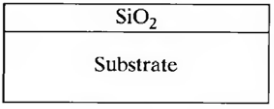
\includegraphics[scale=0.4]{a.png}

  \caption{SiO$_2$ 증착}
  \label{fig:a}
\end{figure}

Cleaning 과정 이후에 웨이퍼는 barrier layer로 덮인다. 이 때 주로 SiO$_2$ 혹은 Si$_3$N$_4$를 이용한다.

\subsubsection{Photoresist application}
\begin{figure}[htbp]
  \centering
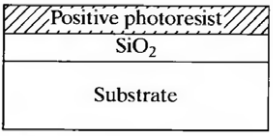
\includegraphics[scale=0.4]{b.png}

  \caption{감광 물질은 SiO$_2$ layer 위에 코팅된다.}
  \label{fig:b}
\end{figure}
SiO$_2$ layer가 구성되면 웨이퍼는 다시 감광 물질로 덮인다. 감광 물질이 잘 부착되기 위해서는
표면이 깨끗하고 건조해야 하지만 이 감광 물질이 잘 붙지 않는 문제가 흔히 발생한다. 이를 해결하기
위해, 접착력을 높여주는 물질로 HMDS를 이용한다. 감광 물질은 주로 액체이기 때문에 웨이퍼를 진공에서
고속으로 회전시켜 감광 물질을 접착시킨다(FIG.~\ref{fig:b}). 

\subsubsection{Soft baking}
Soft baking은 감광 물질의 접착력을 높이고 접착되지 않은 감광 물질을 제거하기 위한 건조 과정이다.
5~30분 동안 60~100$^\circ$C의 온도에서 진행한다.

\subsubsection{Align masks}
Photo mask에는 복잡한 패턴이 새겨져 있어 이를 웨이퍼에 옮기는 과정을 거쳐야 한다. Photo mask가 정확한
위치에 패턴을 옮겨야 하므로 mask들의 위치를 정렬하는 과정을 거친다.

\subsubsection{Photoresist exposure and development}

\begin{figure}[htbp]
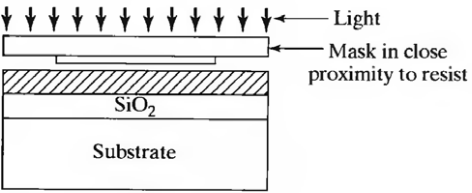
\includegraphics[scale=0.4]{c.png}
\caption{웨이퍼에 옮겨야할 패턴이 mask에 새겨져 있으며 감광 물질의 종류에 따라 mask에 패턴이 새겨진
 방식이 달라진다.}
\label{fig:c}
\end{figure}

Mask를 정렬했다면 감광 물질들은 mask를 통해 강한 자외선에 노출된다. 감광 물질들이 자외선에 노출된 부분들은
SiO$_2$가 추후에 제거될 부분들이다. 자외선에 노출된 감광 물질들은 아래층에 존재하는 SiO$_2$가 노출되도록
씻겨 내려간다. 이렇게 씻겨 내려가는 감광 물질을 positive resist라고 부르며 이 종류의 감광 물질을 사용할 때
mask는 웨이퍼의 표면에 남아 있어야 할 패턴을 포함한다(FIG.~\ref{fig:d}). 

\begin{figure}[htbp]
  \centering
  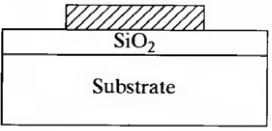
\includegraphics[scale=0.4]{d.png}
  \caption{Positive photoresist의 경우 자외선에 노출된 부분이 씻겨진다.}
    \label{fig:d}
  \end{figure}
이와 반대로 작용하는 negative resist는 자외선에 
노출되지 않은 부분이 씻겨 내려가며 이 종류의 감광 물질을 사용할 때 mask는 웨이퍼의 표면에서 제거되어야 할
패턴을 포함한다. Negative resist는 IC 회로를 구성하는데 주로 사용되며 positive resist는 비교적 작은 스케일의
구조를 다루기에 적함하다(FIG.~\ref{fig:pattern}).


\begin{figure}[htbp]
  \centering
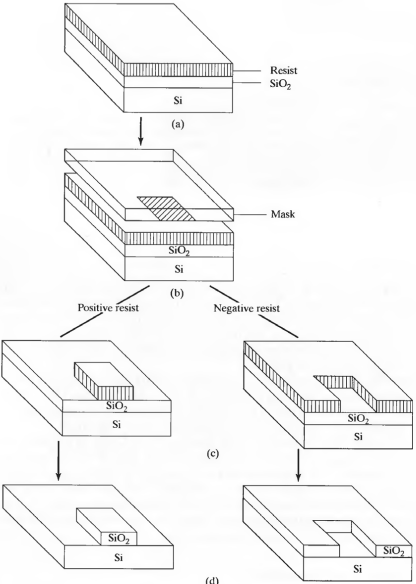
\includegraphics[scale=0.5]{pattern.png}

  \caption{Positive resist와 negative resist를 사용할 때 패턴을 새기는 과정}
  \label{fig:pattern}
\end{figure}

\subsubsection{Hard baking}
자외선에 감광 물질을 조사하고 SiO$_2$ layer를 노출시켰으면 감광 물질을 더 단단하게 하고
웨이퍼에 대한 접착력을 향상시키기 위해 다시 한번 건조, 가열 과정을 거친다.
20~30분 동안 120~180$^\circ$C의 온도에서 진행한다.

\subsubsection{Etch windows in barrier layer}

\begin{figure}[htbp]
  \centering
  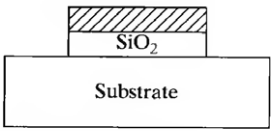
\includegraphics[scale=0.4]{e.png}
  \caption{Etching을 통해 노출된 SiO$_2$는 제거된다.}
    \label{fig:e}
  \end{figure}

Etching은 감광 물질에 덮여있지 않은 부분의 SiO$_2$을 깎아내는 과정으로 wet chemical etching과  
dry plasma etching이 있다(FIG.~\ref{fig:e}).
\begin{itemize}
  \item[A. ] Wet chemical etching은 웨이퍼를 용액에 담그는 방식으로 플루오린화 수소산(HF)가 포함된
  용액을 사용한다. 실온에서 플루오린화 수소산이 감광 물질이나 웨이퍼를 깎는 속도보다 SiO$_2$를 깎는 속도가
  더 빠르다는 점이 이용한다. 물질을 깎는 비율이 온도에 의존하기 때문에 온도를 세밀하게 관리해야 한다.
  Wet chemical etching의 단점 중 하나는 모든 방향에서 동등하게 etching이 진행된다는 것이다.
  이는 패턴의 선폭이 감광 물질의 두께와 유사한 길이일 때 중대한 문제가 될 수 있다(FIG.~\ref{fig:wet}).

  \begin{figure}[htbp]
    \centering
  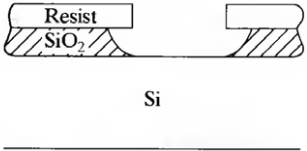
\includegraphics[scale=0.5]{wet.png}
    \caption{Wet chemical etching에 의한 etching은 감광 물질이 씻겨나간 부분보다 더 많은 SiO$_2$를
    깎을 수도 있으며 이는 중대한 문제가 될 수 있다.}
    \label{fig:wet}
  \end{figure}
  

  \item[B. ] Dry plasma etching은 적은 양의 반응 가스만을 필요로 하는 방법으로 플라즈마를 이용한다.
  Wet chemical etching과 달리 undercutting이 발생하는 문제를 피할 수 있다.
  
  
\end{itemize}

\subsubsection{Remove photoresist}
감광 물질은 감광 물질의 접착력을 잃도록 하는 액체를 이용하여 제거한다(FIG.~\ref{fig:f}).
\begin{figure}[htbp]
  \centering
  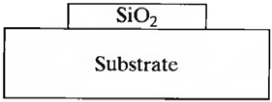
\includegraphics[scale=0.4]{f.png}
  \caption{Ecthing 이후 감광 물질을 제거한 모습}
    \label{fig:f}
  \end{figure}

  \subsection{Depostion}
  Deposition은 다양한 금속을 웨이퍼의 표면에 얇게 쌓는 과정이다.
  \subsubsection{Sputtering}
  Sputtering은 목표지점에 이온을 강하게 충돌시켜 depositoin하는 방법이다. 주로 Ar$^+$가 쓰인다.
  이번 실험에서는 구리 이온을 이용한다.
  이온은 충돌하며 deposition이 발생하는 물질로 운반된다. Sputtering으로 deposition하기 위해
  넘어야 할 threshold energy가 존재하여 입사시키는 이온의 energy를 이 값보다 크게 해야 한다.
  \subsubsection{Chemical vapor deposition}
  Chemical Vapor Deposition(CVD)은 기체 화합물의 반응이나 열을 이용해 표면에 얇게 쌓는 방법이다.
  CVD reactor는 여러 종류가 있으며 APCVD, LPCVD, PECVD가 대표적이다(FIG.~\ref{fig:CVD}). 
  APCVD(Atmospheric Pressure CVD)는 
  silicon dioxide passivation의 deposition에 사용되며 반응 기체의 높은 흐름율을 필요로 한다.
  LPCVD(Low-Pressure CVD)는 
  높은 온도와 낮은 압력을 필요로 하며 polysilicon, silicon dioxide, 
  silicon nitride의 deposition에 사용된다. 
  PECVD(Plasma-Enhanced CVD)는 plasma를 이용해 낮은 온도에서도
  반응이 일어나도록 한다.

  \begin{figure}[htbp]
    \centering
  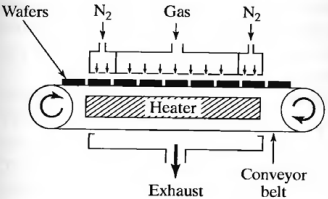
\includegraphics[scale=0.5]{APCVD.png}
    \caption{APCVD reactor}
    \vspace{0.5cm}
  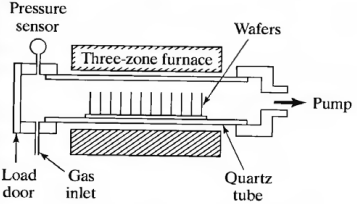
\includegraphics[scale=0.5]{LPCVD.png}
    \caption{LPCVD reactor}
    \vspace{0.5cm}
    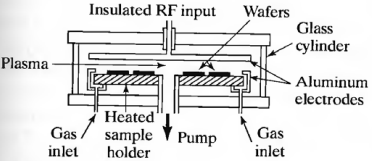
\includegraphics[scale=0.5]{PECVD.png}
    \caption{PECVD reactor}


    \label{fig:CVD}
  \end{figure}



\subsection{Experimental Methods}
\begin{itemize}
  \item[1. ]
  먼저 실험에 필요한 장비들을 아세톤과 알코올로 세척한다. 세척 후 블로워를 이용하여 건조시킨다.
  이번 실험의 장비 세척을 실험 결과에 많은 영향을 미치므로 보다 세심하게 세척해야 한다.
  \item[2. ]
  웨이퍼에 감광 물질을 도포한다. 도포 과정은 스핀 코터를 이용하여 진행한다. 감광 물질은 자외선에
  반응하기 때문에 옐로우룸에서 진행한다. 
  \begin{itemize}
    \item[a. ]  스핀 코터는 1000RPM 부터 4000RPM까지 1000 단위로 
    높여가면서 진행하며 각 RPM에 대한 RamP와 Time 값은 모두 10으로 설정한다. 
    \item[b. ] 스핀 코터를 위 조건으로 세팅하고 Vacuum 버튼을 눌러 웨이퍼를 고정시킨다.
    \item[c. ] 웨이퍼가 고정되면 스포이드를 이용하여 감광 물질 도포를 시작한다. 이 때 기포가 발생하지 않도록
    주의해야하며 도포 이후에도 옐로우룸 밖에서 자외선이 들어오지 않도록 한다.
  \end{itemize}
  \item[3. ]
  웨이퍼를 소프트 베이킹한다. 베이킹 온도는 130{$^\circ$}C이다.
  \item[4. ]
  웨이퍼에 자외선을 노광한다.
  \begin{itemize}
    \item[a. ]
    UV 노광 장비의 본체, UV 램프, 노광 장비 순으로 전원을 인가한다. 
    컴퓨터의 프로그램을 켜면 UV 램프의 전원을 킬 수 있다. 전원을 킨 후
    3.5 ~ 3.7A로 안정될 때 까지 대기한다. 안정화가 완료되면 stable 표시가 화면에 나타난다.
    \item[b. ]
    Mask Holder Lock 버튼을 눌러 잠금을 해제하고 마스크를 넣는다. 마스크를 고정하기 위해 
    Mask Vacuum 버튼을 눌러야 한다.
    \item[c. ]
    Sample stage에 웨이퍼를 올린다. 웨이퍼를 고정하기 위해 Sample Vacuum 버튼을 눌러야 한다.
    \item[d. ]
    Aligner 위 아래쪽에서 $x$, $y$, $z$축 rotation을 조정할 수 있다. 이는 마스크의 위치를
    조절하는데 사용한다.
    \item[e. ]
    준비가 끝나면 position을 exposure로 바꾸어주고 exposure 버튼을 눌러 노광을 진행한다.
    노광이 끝나면 Sample Vacuum을 해제하고 웨이퍼를 꺼낸다.
  \end{itemize}
  \item[5. ]
  노광이 끝나면 현상액으로 웨이퍼를 현상한다. 현상이 끝나면 증류수로 현상액을 제거하고 블로워로
  건조시킨다.
  \item[6. ]
  웨이퍼를 하드 베이킹하여 밀착력을 높인다.
  \item[7. ]
  하드 베이킹이 끝나면 금속을 증착시킨다. 사용되는 금속은 구리이며 증착기를 이용한다.
  \begin{itemize}
    \item[a. ]
    증착기 위에 웨이퍼를 올리고 테이프로 고정한 후 증착기에 전원을 인가한다.
    \item[b. ]
    Cycle 버튼을 눌러 증착기를 작동시키면 금속 플레이트가 웨이퍼 위에 쌓인다. 
    Cycle 버튼이 2번 깜박이면 버튼을 두번 눌러서 증착기를 껐다 킨다. 
    \item[c. ]
    증착이 완료되면 전원을 끄고 진공이 풀린 후에 웨이퍼를 꺼낸다.
  \end{itemize}
  \item[8. ]
  박리 과정을 진행하여 감광 물질을 걷어낸다. 박리는 웨이퍼를 아세톤에 5분 가량 담구어 진행한다.
\end{itemize}

\nocite{*} 
\bibliography{ref}



%\begin{thebibliography}{9}
%\end{thebibliography}

\vfill
\end{document}